Unsere Webseite besteht aus statischen Inhalten wie beispielsweise der Menuführung, die offen im HTML-Dokument liegen und Inhalten, die dynamisch mit Daten aus der Datenbank gefüllt werden: Profile, Chats, Nachrichten. Um diese Daten bereitstellen zu können, ist eine Schnittstelle zwischen Datenbank und Frontend notwendig. 

Wir haben uns für GraphQL entschieden, weil... %TODO fill

\section{GraphQL erklärt}
https://www.youtube.com/watch?v=eIQh02xuVw4

\section{Overfetching und Underfetching}
Unter Overfetching versteht man, dass bei einer Anfrage mehr Daten zurückgegeben werden, als benötigt werden.
Beim Underfetching werden von einem Endpunkt nicht genug Daten zur verfügung gestellt, wodurch mehrere Anfragen erstellt werden müssen.
In beiden Fällen entstehen - durch mehr benötigte Bandbreite oder mehr Anfragen - Leistungseinbuße, die als Folge längere Antwortzeiten und höhere Serverkosten beinhalten.

In klassischen REST-APIs muss für jede Anfrage ein eigener Endpunkt erstellt werden. In einer perfekten Konfiguration bestehen genau die Endpunkte, um exakt die benötigten Daten abfragen zu können. Diese perfekte Konfiguration ist jedoch praxisfern, Anforderungen und damit angefragte Daten verändern sich in einem Projekt dauernd, zudem kostet es Ressourcen, jeden einzelnen Endpunkt zu betreiben und zu warten. 

GraphQL löst dieses Problem, da bei jeder Anfrage genau definiert werden kann, welche Daten erfragt werden sollen und welche Endpunkte dafür verwendet werden. 
%TODO Beispiel-Bild von GQL-Afrage

\section{Typisierung}
Stark definierte Datentypen verringern das Risiko einer Fehlkommunikation zwischen Client und Server.

\section{Dokumentation}
GraphQL erlaubt es, jeden Endpunkt und jedes Anfragefeld zu dokumentieren. Dies erleichtert es dem Frontend, die richtigen Endpunkte für ihre Anfrage zu verwenden.

\section{GraphiQL}
GraphiQL ist eine browserbasierte Programmierumgebung, mit der Programmierer Zugriff auf die GraphQL-Dokumentation der Webseite haben. Dies erleichtert die Programmierung im Frontend.

\section{}







Schnittstelle zur Kommunikation zwischen Datenbank und frontend

Graphql vs REST

Verwendete packages
Apollo
Graphql Playground
graphql-compose(-mongoose)

Für einige Daten Authentifizierung und Autorisierung benötigt

Fazit


Mit GraphQL sind APIs schnell, flexibel und einfach für Entwickler.
\\ \\
Laut dem 2020 State of the API Report von Postman.com steht GrapQL an fünfter Stelle der spannendsten Technologien für 2021.
{Vgl. u.a. \cite{PM1}}

Im Hinblick auf die Art und Weise, wie Abfragen an den Server mithilfe von 
\\ GraphQL behandelt werden können, sind folgende Aspekte zu beachten.


  \end{itemize}

  \footnote{Vgl. u.a. \cite{RH1}}
\end{quote}

\subsubsection{GraphQL Playground}
Mit GraphQL Playground haben wir die Möglichkeit, alle Abfragen und Mutationen zu testen. Wir erhalten Zugriff auf relevante Informationen wie verfügbare Felder und deren Datentyp. Diese Informationen werden aktualisiert, wenn der Servercode geändert wurde. Dadurch wurde eine aktuelle API-Dokumentation gewährleistet. Für unser Projekt war es sehr praktisch und hat die Kommunikation als Entwickler effizienter gemacht.
\\
\begin{center}
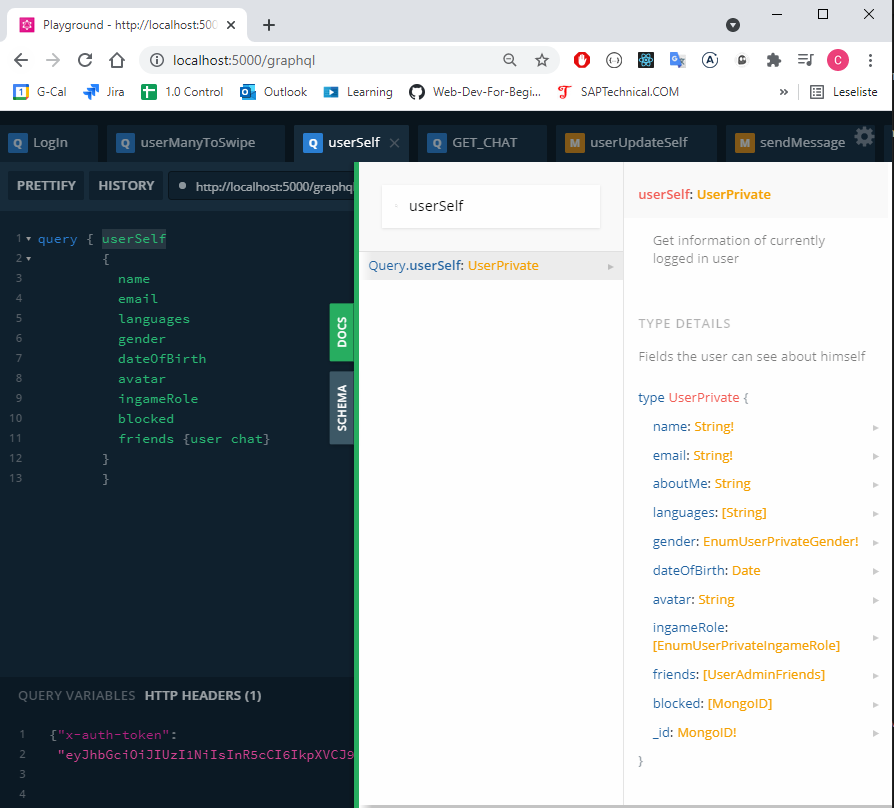
\includegraphics[scale=0.60]{GraphQL_Playground}\label{fig:GraphQL_Playground}
\end{center}
\textbf{Abbildung \autoref{fig:GraphQL_Playground}:}
Genau derselbe Code wird für die Abfrage von Benutzerinformationen später verwendet.
\newpage

\subsection{Implementierung der Serveranfragen mit GraphQL}
Alle Abfragen und Mutationen wurden in einem separaten Ordner gesammelt.
Damit soll eine saubere Struktur des Codes gewährleistet werden.
Diese wurden für die spätere Verwendung in den React-Komponenten exportiert.

Mithilfe der Hooks useQuery bzw. useMutation von Apollo Client wurden die Lese- und Schreibabfragen durchgeführt.
\\\\
\textbf{Apollo Client}\\
Warum haben wir uns für Apollo entschieden? Was ist ApolloClient?
TODO
%Coming...
\newpage

\subsubsection{Leseabfrage}
Nachdem eine Abfrage exportiert wurde, ist sie bereit, in einer React-Komponente \\
importiert und angewendet zu werden.

\begin{lstlisting}
import { GET_MY_INFO } from "./GraphQL/Queries"
import { useQuery } from "@apollo/client"

const { loading, error, data } = useQuery(
GET_MY_INFO,
ContextHeader(token),
)
//Code-Auszug in frontend/src/App.js

\end{lstlisting}
Die Konstante ContextHeader enthält das Token in der Struktur, die erforderlich ist, um die Abfrage nur dann stellen zu können, wenn der Benutzer dazu berechtigt ist.
\\
Sollte das Token einen undefinierten Wert, null oder ungültig enthalten, wird der Server ein Fehler zurückgegeben.
\\
Der useQuery Hook liefert ein Ergebnisobjekt, welches eine der folgenden Optionen zurückgibt.
\\\\
\textbf{loading:}\\
Ein boolescher Wert, der angibt, ob die Abfrage in Bearbeitung ist.
Wenn loading wahr ist, ist die Anfrage noch nicht abgeschlossen. Typischerweise kann diese Information verwendet werden, um einen Lade-Spinner anzuzeigen.
\\\\
\textbf{error:}\\
Ein Laufzeitfehler mit den Eigenschaften von GraphQL Errors und network Error.
Dieses enthält Informationen darüber, was bei der Abfrage fehlgeschlagen  ist.
\\\\
\textbf{date:}\\
Ein Objekt, das das Ergebnis der GraphQL-Abfrage enthält.
\\Es enthält die tatsächlichen Daten vom Server.
\\
\newpage

%TODO: AUCH MUTATIONS ZEIGEN
\subsubsection{Mutationen}
\subsubsection{Subscriptions}

TODO after receiving feedback about the rest.

\newpage
\subsection{Axios}
Zusätzlich zu den GraphQL-Abfragen wurde eine Post-Anfrage mit Axios bereitgestellt.
Mit dieser war es möglich, Bilder auf die S3 Speicher von AWS hochzuladen.

\begin{quote}
  Axios ist ein Promise-basierter HTTP-Client für node.js und den browser. Auf der Server-Seite wir das modul http verwendet, während im Browser XMLHttpRequests (ajax) ausgeführt werden.
\end{quote}\footnote{Vgl. u.a. \cite{AX1}}

\begin{lstlisting}
    function disableBtn() {
        const uploadBtn = document.getElementById("uploadBtn")
        uploadBtn.disabled = true
        uploadBtn.style.background = "#000000"
      }
    
      function fileUploadHandler() {
        errored ? 
         disableBtn()
         /*
        Tritt ein Fehler auf, wird die Abfrage nicht gesendet und der Knopf deaktiviert 
        Ein Fehler tritt auf, wenn die Datei zu gross ist oder oder wenn sie ein ungueltiges  Format hat
        */
        :
        console.log("uploading pic...", file?.name)
        const fd = new FormData()
        /* avatar ist der Name der Datei, die hochgeladen wird
          file ist der zu sendende  Wert */
        fd.append("avatar", file)  
    
        axios
          .post(urlAvatar, fd, {
            headers: {
              "x-auth-token": TOKEN,
            },
          })
          .then((res) => {
            setState((state) => ({ ...state, avatar: res?.data?.location }))    
            //In location finden wir die URL fuer das gerade hochgeladende Bild 
          })
      }\end{lstlisting}

%Das HTML-Eingabefeld „input“ wurde folgendermaßen definiert.
%\begin{lstlisting}
 %   <input type="file" onChange={fileSelectedHandler} />
%\end{lstlisting}


Das Format der hochzuladenden Dateien wurde limitiert, damit nur zulässige Dateien an den Server gesendet werden.
\begin{lstlisting}
    const admittedImageFormats = ["png", "jpg", "jpeg"]
\end{lstlisting}

Die Größe der hochzuladenden Datei wurde um 1 MB abgegrenzt.
Durch die Eigenschaft „size“ der ausgewählten Datei konnten wir auf die Größe der Datei zugreifen.
\begin{lstlisting}
    const imageSize = e.target.files[0].size
\end{lstlisting}
